\section{Applying Online-PCA}

\subsection{Novelty filter}

\mode<presentation>{
\begin{frame} 
    \begin{center} \huge
        \secname
    \end{center}
    Same as PCA
    Example Application: Novelty filter
\end{frame}
}

\begin{frame}

Applying online PCA for detecting outliers - identifying observations with unusual features. 

\slidesonly{
\begin{center}
	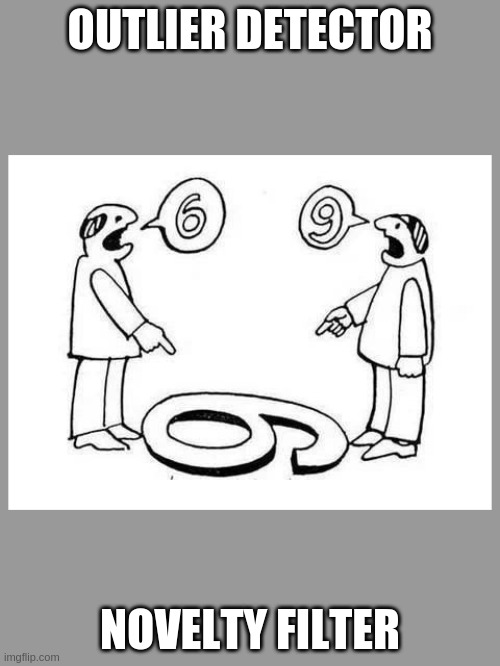
\includegraphics[width=0.3\textwidth]{img/meme_outlier_novelty}%
\end{center}
}
Calling it an ``outlier'' or a point with `novel'' features depends on the context. But they are essentially the same.

Can also be done using ``standard'' or ``batch'' PCA.

\end{frame}

\begin{frame}\frametitle{\subsecname}

\only<1>{
\question{What are the PCs with smallest eigenvalues useful for?}
}

\pause 
\question{Can we modify online PCA by learning the PCs in reverse order (i.e. PCs with smallest eigenvalues first?}\\

\only<3>{
\slidesonly{
\begin{center}
	
\includegraphics[width=0.3\textwidth]{img/meme_yesyoucan}%
\end{center}
}
}

\end{frame}

\subsubsecname{Novelty Filter with normalization}

\begin{frame}\frametitle{\subsubsecname}

\notesonly{- Yes by using the}

	\begin{block}{Anti-Hebbian rule:}
				\begin{equation}
				\Delta w_j = \overbrace{-}^{\substack{	\text{``Anti''-} \\ \text{Hebbian} }} \varepsilon y^{(\alpha)} x_j^{(\alpha)}
				\end{equation}
	\end{block}
	
	Not prone to diveregence but $\vec w$ will become smaller and smaller.
	\pause
	
	Normalization needed:
	
	\begin{equation}
		\Delta \vec{w} = - \varepsilon  \frac{y^{(\alpha)} \left\{ \vec{x}^{(\alpha)} - y^{(\alpha)} \vec{w} \right\}}{|{\vec{w} - \varepsilon y^{(\alpha)} \left\{ \vec{x}^{(\alpha)} - y^{(\alpha)} \vec{w} \right\}}|}
	\end{equation}
	
	Anti-Hebbian version of Oja's rule also (cf. lecture slides)

\end{frame}


\begin{frame}

\question{Are the other ways to learn a novelty filter without PCA?}

\pause

- Yes, through linear regression:

\end{frame}

\newpage

\subsubsection{Novelty Filter and linear regression}

\begin{frame}\frametitle{\subsubsecname}
	\svspace{-3mm}

\begin{center}
\notesonly{
\hspace{-10mm}
}
\begin{minipage}{0.45\textwidth}
	\begin{center}
		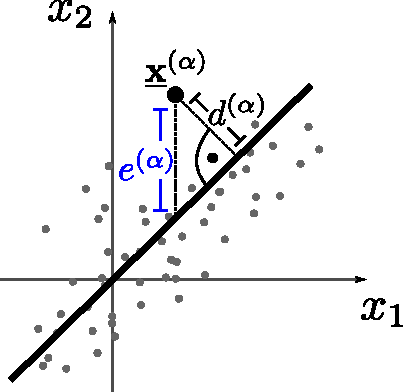
\includegraphics[width=0.6\textwidth]{img/linear_regression}%
		%\captionof{figure}{Ordinary least squares}
	\end{center}
	\svspace{-5mm}
	
	\begin{block}{ordinary least squares:}
	\svspace{-2mm}
		\begin{equation}
		\frac{1}{p} \sum_{\alpha = 1}^{p} \left( {\color{blue}e^{(\alpha)}} \right)^2 \eqexcl \min_{\vec w}
		\end{equation}
	\end{block}
\end{minipage}
\slidesonly{
\hspace{5mm}
}
\notesonly{
\hspace{2mm}
}
\visible<2>{
\begin{minipage}{0.45\textwidth}
	\begin{center}
		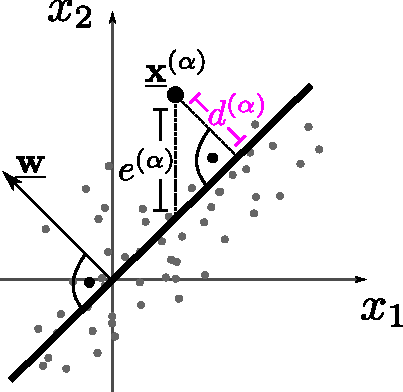
\includegraphics[width=0.6\textwidth]{img/linear_regression_a}%
		%\captionof{figure}{Total least squares}
	\end{center}
	\svspace{-5mm}
	
	\begin{block}{total least squares:}
	\svspace{-2mm}
			\begin{equation}
				\frac{1}{p} \sum_{\alpha =1}^{p} \left( {\color{magenta}d^{(\alpha)}} \right)^2 \eqexcl \min_{\vec w}
			\end{equation}
		\end{block}
\end{minipage}
}
\end{center}

\svspace{-1mm}

\underline{Assumptions}:\\




\svspace{-1mm}

\notesonly{
	\resizebox{0.8\textwidth}{!}{%
	\begin{tabular}{|l|l|}
	\hline 
	ordinary least squares		  &  total least squares
	\\ \hline
	$\leadsto$ noise along $x_2$ only		  &  $\leadsto$ same variance noise\\ \hline
	$\leadsto$wrong if data points are also noisy along $x_1$ & $\leadsto$ centered data $\rightarrow \vec{w}^\top\vec{x} = 0$ 
	\\ \hline
	\end{tabular}%
	}
}

\slidesonly{	
\begin{center}
\begin{minipage}{\slidesonly{0.45}\notesonly{0.3}\textwidth}
		\begin{itemize}
			\itl noise along $x_2$ only
			\itl wrong if data points are also noisy along $x_1$
		\end{itemize}
\end{minipage}
\hspace{5mm}
$\Bigg|$
\visible<2>{
\begin{minipage}{\slidesonly{0.45}\notesonly{0.3}\textwidth}
		\begin{itemize}
			\itl same variance noise
			\itl centered data $\rightarrow \vec{w}^\top\vec{x} = 0$ 
		\end{itemize}
\end{minipage}
}
\end{center}
}


%- (cf. slides 1.2 \#23-\#25.)


\end{frame}

\section{PCA vs. online PCA}

\begin{frame}\frametitle{\secname}

\underline{Common properties:}

\begin{itemize}
\item assume the data is centered
\item sensitive to the scales of the individual variables
\item for stationary data, both converge to the same solution
\item limited to linear correlations between the variables (cf. Kernel PCA to account for non-linear correlations)
\end{itemize}

\pause

\question{PCA vs. online PCA. How to choose?}\\

\only<2>{
\slidesonly{
\begin{center}
	
\includegraphics[width=0.2\textwidth]{img/mem_pca_vs_online_pca}%
\end{center}
}
}

\pause

- staionarity of the data\\
- can I fit all the data into memory?


\end{frame}
